\documentclass[pdflatex,compress,mathserif]{beamer}

%\usetheme[dark,framenumber,totalframenumber]{ElektroITK}
\usetheme[darktitle,framenumber,totalframenumber]{ElektroITK}

\usepackage[utf8]{inputenc}
\usepackage[T1]{fontenc}
\usepackage{lmodern}
\usepackage[bahasai]{babel}
\usepackage{amsmath}
\usepackage{amsfonts}
\usepackage{amssymb}
\usepackage{graphicx}
\usepackage{multicol}
\usepackage{lipsum}

\newcommand*{\Scale}[2][4]{\scalebox{#1}{$#2$}}%

\title{PEMODELAN JARINGAN KOMUNIKASI}
\subtitle{Routing Fundamentals}

\author{Tim Dosen Pengampu}

\begin{document}

\maketitle

\section{Connected and Local Routes}

\begin{frame}
	\frametitle{Router Functions}
	\begin{itemize}
		\item A router has two main functions:
		\begin{itemize}
			\item Determining the best path to available networks
			\item Forwarding traffic to those networks
		\end{itemize}
	\end{itemize}
\end{frame}

\begin{frame}
	\frametitle{The Routing Table}
	\begin{itemize}
		\item The best available path or paths to a destination network are listed in a router’s routing table and will be used for forwarding traffic
		\item A routing table consists of directly connected networks and routes configured statically by the administrator or dynamically learned through a routing protocol.
	\end{itemize}
\end{frame}

\begin{frame}
	\frametitle{Connected and Local Routes}
	\begin{itemize}
		\item The administrator configures IP addresses on the router's interfaces
	\end{itemize}
	\texttt{interface FastEthernet0/0 \\
		ip address 10.0.0.1 255.255.255.0 \\
		interface FastEthernet1/0 \\
		ip address 10.0.1.1 255.255.255.0 \\
		interface FastEthernet2/0 \\
		ip address 10.0.2.1 255.255.255.0} 
	\begin{center}
		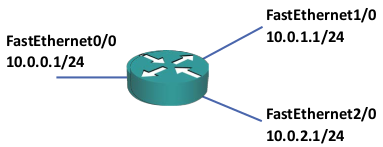
\includegraphics[width=0.5\linewidth]{img/img01}
	\end{center}
\end{frame}

\begin{frame}
	\frametitle{show ip route - Connected Routes}
	\begin{itemize}
		\item This will automatically enter connected routes into the routing table:
		\item[] \texttt{\footnotesize R1\#sh ip route\\
			C $ \quad $ 10.0.0.0/24 is directly connected, FastEthernet0/0 \\
			C $ \quad $ 10.0.1.0/24 is directly connected, FastEthernet1/0 \\
			C $ \quad $ 10.0.2.0/24 is directly connected, FastEthernet2/0}
		\item If any traffic for the 10.0.0.0/24 network is received in another interface on the router, it will forward it out interface FastEthernet0/0
	\end{itemize}
	\begin{center}
		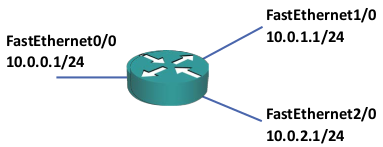
\includegraphics[width=0.5\linewidth]{img/img01}
	\end{center}
\end{frame}

\begin{frame}
	\frametitle{show ip route - Local Routes}
	\begin{itemize}
		\item From IOS 15, local routes will also be added to the routing table
		\item Local routes always have a /32 mask and show the IP address configured on the
		interface
		\item[] \texttt{\footnotesize R1\#sh ip route\\
			L $ \quad $ 10.0.0.1/32 is directly connected, FastEthernet0/0\\
			L $ \quad $ 10.0.1.1/32 is directly connected, FastEthernet1/0\\
			L $ \quad $ 10.0.2.1/32 is directly connected, FastEthernet2/0}
	\end{itemize}
	\begin{center}
		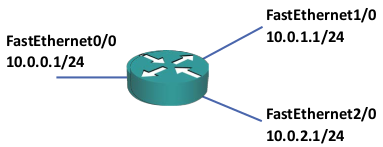
\includegraphics[width=0.5\linewidth]{img/img01}
	\end{center}
\end{frame}

\begin{frame}
	\frametitle{Lab}
	\begin{center}
		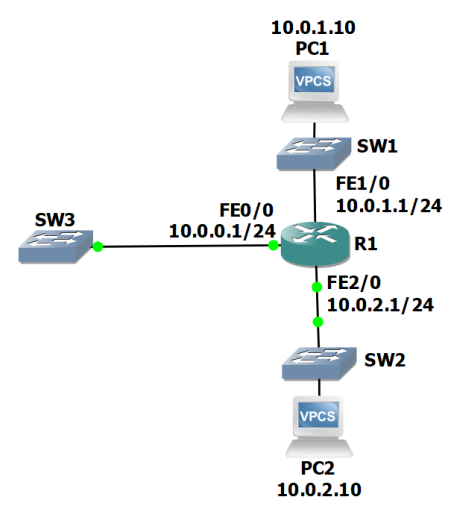
\includegraphics[width=0.5\linewidth]{img/img02}
	\end{center}
\end{frame}

\section{Static Routes}

\begin{frame}
	\frametitle{Static Routes}
	\begin{itemize}
		\item If a router receives traffic for a network which it is not directly attached to, it needs to know how to get there in order to forward the traffic
		\item An administrator can manually add a static route to the destination, or the router can learn it via a routing protocol
	\end{itemize}
	\begin{center}
		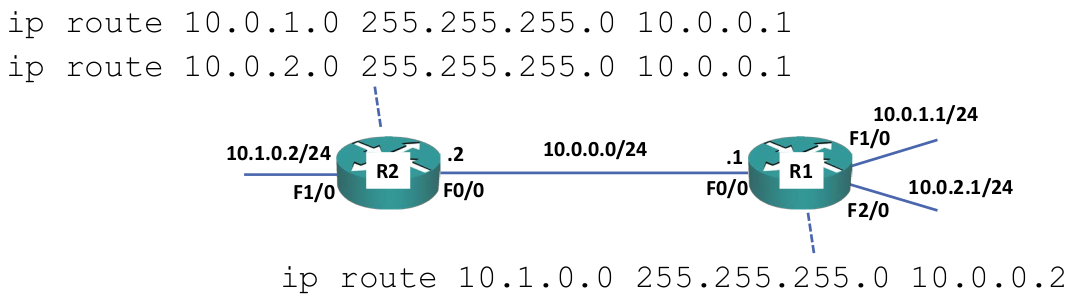
\includegraphics[width=\linewidth]{img/img03}
	\end{center}
\end{frame}

\begin{frame}{Static Routes}
	\begin{center}
		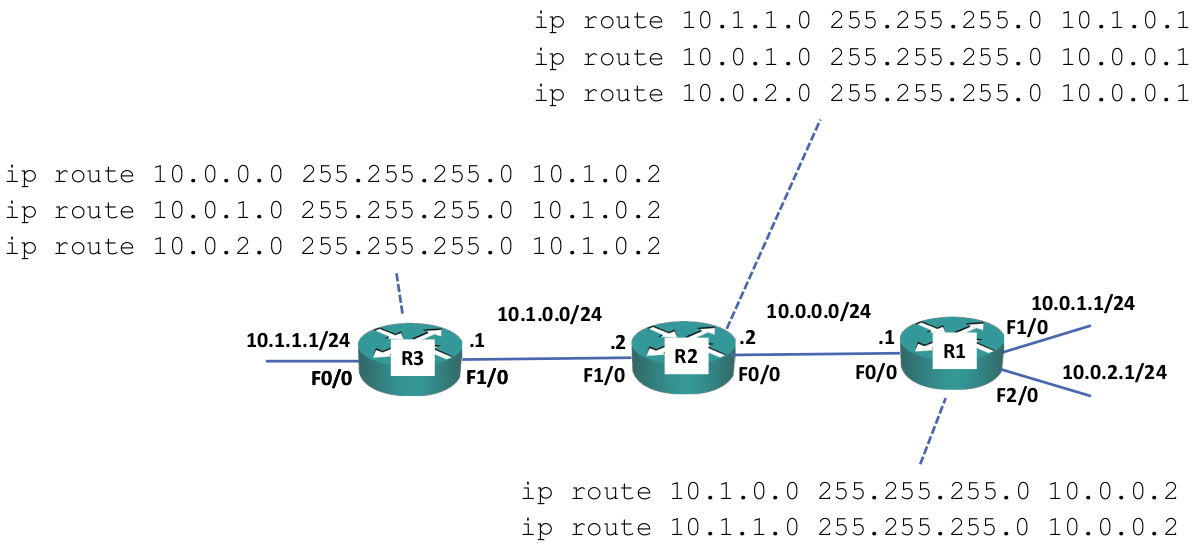
\includegraphics[width=\linewidth]{img/img04}
	\end{center}
\end{frame}

\begin{frame}
	\frametitle{Lab}
	\begin{center}
		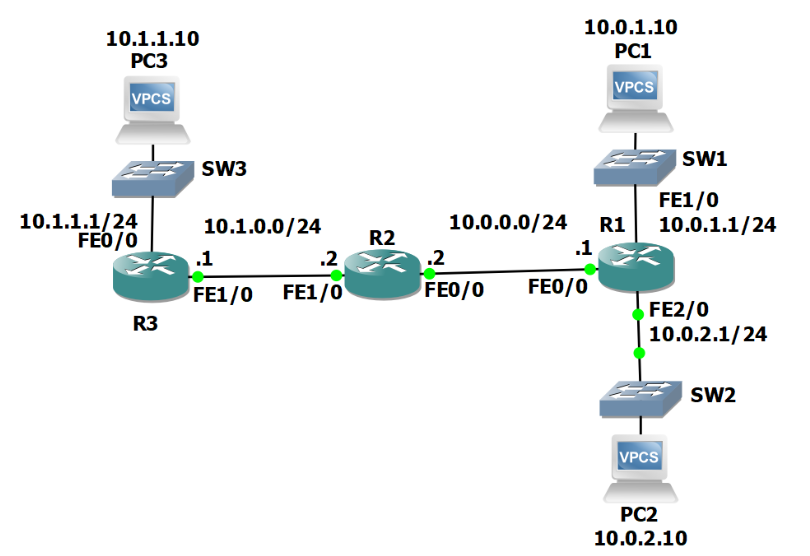
\includegraphics[width=0.8\linewidth]{img/img05}
	\end{center}
\end{frame}

\section{Summarisation and Default Routes}

\begin{frame}
	\frametitle{Static Routes}
	\begin{itemize}
		\item Routes on R1:
		\begin{itemize}
			\item[] \texttt{ip route 10.1.0.0 255.255.255.0 10.0.0.2}
			\item[] \texttt{ip route 10.1.1.0 255.255.255.0 10.0.0.2}
			\item[] \texttt{ip route 10.1.2.0 255.255.255.0 10.0.0.2}
		\end{itemize}
		\begin{center}
			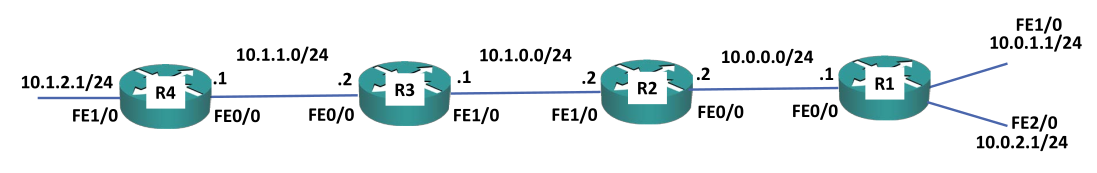
\includegraphics[width=\linewidth]{img/img06}
		\end{center}
	\end{itemize}
\end{frame}

\begin{frame}
	\frametitle{Summary Routes}
	\begin{itemize}
		\item For static routing, summary routes lessen administrative overhead and memory usage on the routers
		\item Routes on R1:
		\begin{itemize}
			\item[] \texttt{ip route 10.1.0.0 255.255.0.0 10.0.0.2}
		\end{itemize}
		\begin{center}
			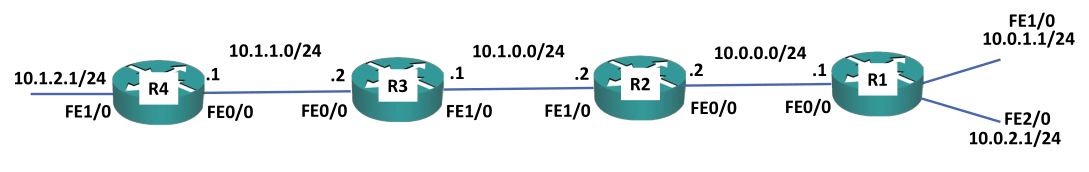
\includegraphics[width=\linewidth]{img/img07}
		\end{center}
	\end{itemize}
\end{frame}

\begin{frame}{Summary Routes}
	\begin{itemize}
		\item Summarisation doesn’t have to be on classful boundaries
		\item To summarise the range 10.1.0.0 to 10.1.3.0:
		\begin{itemize}
			\item[] \texttt{ip route 10.1.0.0 255.255.252.0 10.0.0.2}
		\end{itemize}
		\begin{center}
			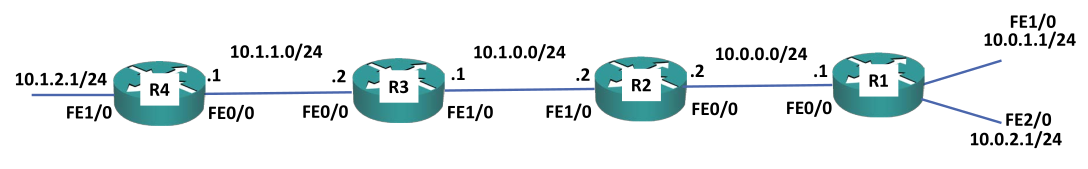
\includegraphics[width=\linewidth]{img/img08}
		\end{center}
	\end{itemize}
\end{frame}

\begin{frame}
	\frametitle{Longest Prefix Match}
	\begin{itemize}
		\item When there are overlapping routes, the longest prefix will be selected
		\begin{itemize}
			\item[] \texttt{ip route 10.1.0.0 255.255.0.0 10.0.0.2}
			\item[] \texttt{ip route 10.1.3.0 255.255.255.0 10.0.3.2}
		\end{itemize}
		\begin{center}
			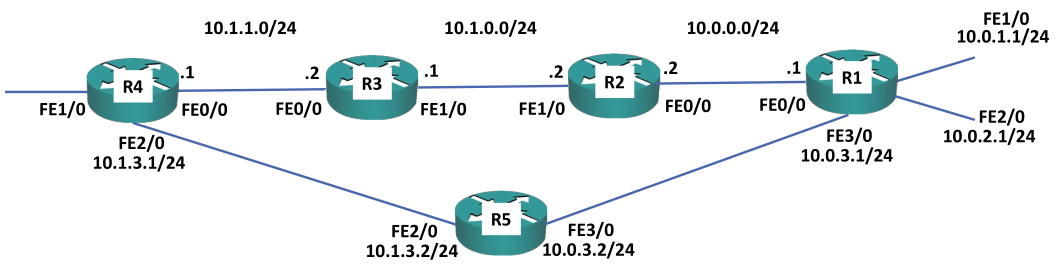
\includegraphics[width=\linewidth]{img/img09}
		\end{center}
	\end{itemize}
\end{frame}

\begin{frame}
	\frametitle{Load Balancing}
	\begin{itemize}
		\item When multiple equal length routes are added for the same destination, the router will add them all to the routing table and load balance between them
		\begin{itemize}
			\item[] \texttt{R1(config)\# ip route 10.1.0.0 255.255.0.0 10.0.0.2}
			\item[] \texttt{R1(config)\# ip route 10.1.0.0 255.255.0.0 10.0.3.2}
		\end{itemize}
		\begin{center}
			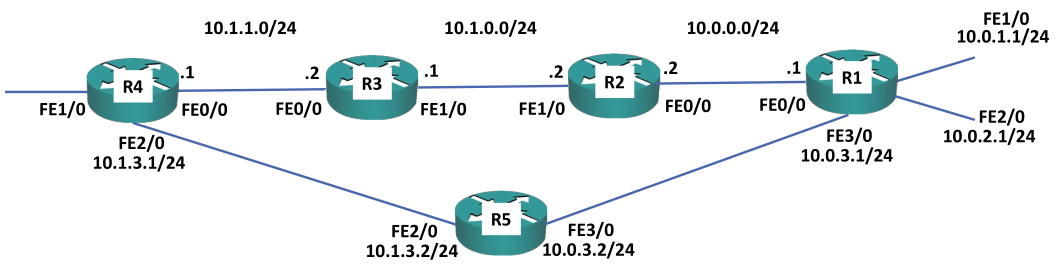
\includegraphics[width=\linewidth]{img/img09}
		\end{center}
	\end{itemize}
\end{frame}

\end{document}
